%\documentclass[border=0pt]{standalone}
\documentclass[preview,varwidth=\maxdimen]{standalone}[2011/12/21]

%\pagestyle{empty}

%\usepackage[papersize={5.0cm,7cm},margin={0pt,0pt,0pt,0pt}]{geometry}

\usepackage{amsmath}

\usepackage{graphicx}
\usepackage{tikz}
\usetikzlibrary{matrix,arrows,shapes}
%% The amssymb package provides various useful mathematical symbols
\usepackage{amssymb}
%% The amsthm package provides extended theorem environments
 \usepackage{amsthm}
 \usepackage{mathrsfs}



\usepgflibrary{shapes.symbols}    
\usepgflibrary[shapes.symbols]    
\usetikzlibrary{shapes.symbols}  
\usetikzlibrary[shapes.symbols]  


\begin{document}

%\begin{figure*}
%\centering
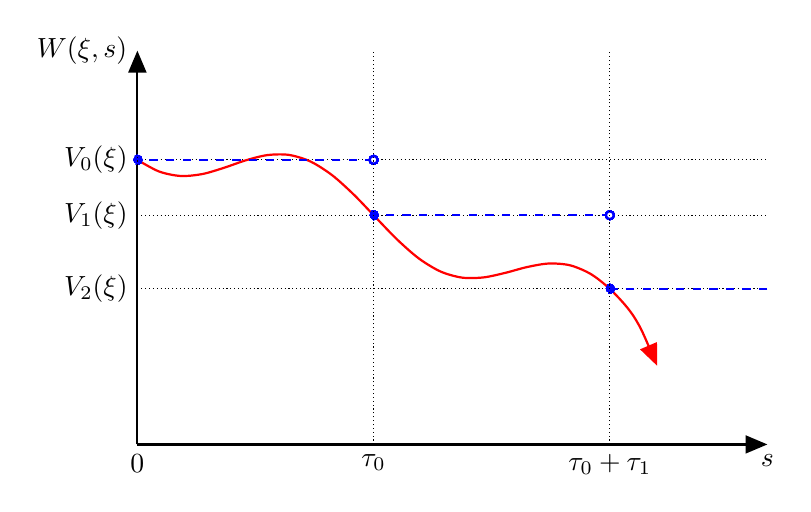
\begin{tikzpicture}[scale=2, >=triangle  45]

%\draw [](0,0) ellipse (70pt and 98pt);

% \draw[thick, <-, color=blue] plot [smooth,tension=.7] coordinates{(4.5,2.9)(3.3,2.3)(2.5,2.5)(1.7,3)(1,2.8)};
 
% \node [] (o) at (0,0){$O$};
 
  \node [ left] (o) at (0,{exp(sqrt(3.3)/2)+.2*sin(3.3*200)-.5}){ {$V_0(\xi)$}};
   \node [ left] (o) at (0,{exp(sqrt(1.8)/2)+.2*sin(1.8*200)-.5}){ {$V_1(\xi)$}};
   \node [ left] (o) at (0,{exp(sqrt(0.3)/2)+.2*sin(0.3*200)-.5}){ {$V_2(\xi)$}};
  
%  \node [ below] (o) at (0,-1.5){ {\tiny$\tau$}};




  \draw[thick,->] (0,0) -- (4,0)node[below]{$s$};
  \draw[thick,->] (0,0) -- (0,2.5)node[left]{$W(\xi,s)$};
    \draw[densely dotted] (0,{exp(sqrt(3.3)/2)+.2*sin(3.3*200)-.5}) -- (4, {exp(sqrt(3.3)/2)+.2*sin(3.3*200)-.5});
    \draw[densely dotted] (0,{exp(sqrt(1.8)/2)+.2*sin(1.8*200)-.5}) -- (4,{exp(sqrt(1.8)/2)+.2*sin(1.8*200)-.5});
     \draw[densely dotted] (0,{exp(sqrt(0.3)/2)+.2*sin(0.3*200)-.5}) -- (4,{exp(sqrt(0.3)/2)+.2*sin(0.3*200)-.5});

\draw (3,0) node[below]{$\tau_0+\tau_1$};
%\draw (0,1) node[left]{$|x(0)|$};
\draw (1.5,0) node[below]{$\tau_0$};
%\draw (2.3,0) node[below]{$t_{i-1}$};
\draw (0,0) node[below]{$0$};
%\draw (3.8,0) node[below]{$t_{i+1}$};
%\draw (4.6,0) node[below]{$t_{i+2}$};

%\draw (.6,0) node[below]{$\cdots$};
%\draw (5.5,-0.1) node[below]{$\cdots$};


\draw[red,thick,-,smooth,domain=0:3.3, <-] plot({-\x+3.3},{exp(sqrt(\x)/2)+.2*sin(\x*200)-.5});
%\draw[red,thick,-,domain=0:2.3] plot({\x+3},{exp(\x/2)+.2*sin(\x*200)});

    \draw[dashed, thick, color=blue] plot (1.5,{exp(sqrt(3.3)/2)+.2*sin(3.3*200)-.5}) -- plot [mark=*,mark size=.7pt] (0, {exp(sqrt(3.3)/2)+.2*sin(3.3*200)-.5});
    \draw[dashed, thick, color=blue] plot (3,{exp(sqrt(1.8)/2)+.2*sin(1.8*200)-.5}) -- plot [mark=*,mark size=.7pt](1.5,{exp(sqrt(1.8)/2)+.2*sin(1.8*200)-.5});
     \draw[dashed, thick, color=blue] (4,{exp(sqrt(0.3)/2)+.2*sin(0.3*200)-.5}) -- plot [mark=*,mark size=.7pt](3,{exp(sqrt(0.3)/2)+.2*sin(0.3*200)-.5});

\draw[thick, color=blue] plot [mark=*,mark size=.7pt,mark options={fill=white}](1.5,{exp(sqrt(3.3)/2)+.2*sin(3.3*200)-.5});
\draw[thick, color=blue] plot [mark=*,mark size=.7pt,mark options={fill=white}](3,{exp(sqrt(1.8)/2)+.2*sin(1.8*200)-.5});
% \draw[thick, color=blue] plot [mark=*,mark size=.7pt] (3, {exp(sqrt(3.3)/2)+.2*sin(3.3*200)-.5});
%\draw[thick, color=blue] plot [smooth,tension=.5, mark=*,mark size=.7pt] coordinates{({.5 r}: {1+0.15*.25})} ;
  
  \draw [densely dotted] (1.5,0) -- (1.5,2.5);
  \draw [densely dotted] (0,0) -- (0,2.5);
   \draw [densely dotted] (3,0) -- (3,2.5);
%   \draw [densely dotted] (3.8,0) -- (3.8,3);
%\draw [densely dotted] (4.6,0) -- (4.6,5);

%  \draw[] (5.3,3.3)node[right]{$|x(t)|$};

%\draw[thick,color=red,fill=white] (3,4.181762) circle (1.1pt);
%\draw[thick,color=red,fill=red] (3,1) circle (1.1pt);
%\draw[thick,color=red,fill=red] (0,1) circle (1.1pt);
 
\end{tikzpicture}
%\end{figure*}


\end{document}
